%%%%%%%%%%%%%%%%%%%%%%%%%%%%%%%%%%%%%%%%%
%  A bright and image filled report style, currently set up here for use with ILM report 8600-219.
%  Contains all that is required, glossaries, content management, references and good looks.
%
% The original template (the Legrand Orange Book Template) can be found here --> http://www.latextemplates.com/template/the-legrand-orange-book
% Original author of the Legrand Orange Book Template:
% Mathias Legrand (legrand.mathias@gmail.com) 
%
% Modifications made for ILM specific reporting
% 
%
% License:
% CC BY-NC-SA 3.0 (http://creativecommons.org/licenses/by-nc-sa/3.0/)
%%%%%%%%%%%%%%%%%%%%%%%%%%%%%%%%%%%%%%%%%
 
%%%%%%%%%%%%%%%%%%%%%%%%%%%%%%%%%%%%%%%%%
% How to use this
%
% Upload a file called FrontCover.jpg to become your new front cover - into the Pictures folder
% Upload files called Heading1.jpg, Heading2.jpg etc to become your new chapter headers - into the Pictures folder
% Make sure these images are the right size to fit their locations and use good quality images
%
% Locate the variables below and set your name, title etc.
%
% If you want to change text colour on the front cover, the areas required are commented below
% If you want to modify text and border colours for your chapter headers go into the structure.tex file and replace the name of the colour (set to ) with a new colour name (find and replace ctrl+f will do this for you).
%
% Add all references into references.bib
% Cite these references by using \cite{referenceName}
%
% Commonly used acronyms or industry specific terms should be added to the glossary
% These terms may then be referenced in the text using \gls{termName}
%
% Finally put some answers in there!
%
% 
% Note: This template is set up specifically for ILM reports, it can be modified for other forms of reports
%
%%%%%%%%%%%%%%%%%%%%%%%%%%%%%%%%%%%%%%%%
 
 
%----------------------------------------------------------------------------------------
%	SET THESE VARIABLES!
%----------------------------------------------------------------------------------------

\def\mytitle{Physics - First Tome.} % Title of the ILM project
\def\ILMCode{A friendly approach.} % Unique code for the ILM project

\def\ILMCentreName{ILM centre name } % The name of the centre you're the ILM sitting at
\def\ILMCentreCode{123456/A} % Unique code the centre at which you're sitting the ILM
\def\ILMLevel{3 } % What level are you sitting with the ILM. i.e. 3, 4, 5
\def\reviewer{Reviewer's name} % You may not know this, if not use the centre's name

\def\author{Jaime Andres Torres Bermejo} % Your name.. 
\def\id{github.com/XaurDesu} % Your unique identifier

\def\date{\today } % Today's date 


 
%----------------------------------------------------------------------------------------
%	PACKAGES AND OTHER DOCUMENT CONFIGURATIONS
%----------------------------------------------------------------------------------------

\documentclass[11pt,fleqn]{book} % Default font size and left-justified equations

\usepackage[dvipsnames]{xcolor}

%%%%%%%%%%%%%%%%%%%%%%%%%%%%%%%%%%%%%%%%%
% This is based on the Legrand Orange Book
% Structural Definitions File
%
% The original template (the Legrand Orange Book Template) can be found here --> http://www.latextemplates.com/template/the-legrand-orange-book
%
% Original author of the Legrand Orange Book Template::
% Mathias Legrand (legrand.mathias@gmail.com) with modifications by:
% Vel (vel@latextemplates.com)
%
% Original License:
% CC BY-NC-SA 3.0 (http://creativecommons.org/licenses/by-nc-sa/3.0/)
%
%%%%%%%%%%%%%%%%%%%%%%%%%%%%%%%%%%%%%%%%%
%----------------------------------------------------------------------------------------
%	VARIOUS REQUIRED PACKAGES
%----------------------------------------------------------------------------------------

\usepackage{titlesec} % Allows customization of titles

\usepackage{graphicx} % Required for including pictures
\graphicspath{{Pictures/}} % Specifies the directory where pictures are stored

\usepackage{lipsum} % Inserts dummy text

\usepackage{tikz} % Required for drawing custom shapes

\usepackage[english]{babel} % English language/hyphenation

\usepackage{enumitem} % Customize lists

\setlist{nolistsep} % Reduce spacing between bullet points and numbered lists

\usepackage{booktabs} % Required for nicer horizontal rules in tables

\usepackage{eso-pic} % Required for specifying an image background in the title page

\usepackage{glossaries} %Required to allow the creation of glossary items, allows for referencing within the document

\usepackage[none]{hyphenat} %Stops words which are too long for a line being split over two lines using hyphenation

\usepackage[top=3cm,bottom=3cm,left=3.2cm,right=3.2cm,headsep=10pt,letterpaper]{geometry} % Page margins
\usepackage{algorithm} % Writing nice algorithms
\usepackage{algpseudocode} % Writing pseudocode
\usepackage{longtable} %Tables which may stretch over more than 1 page
\usepackage{rotating} %Rotate images using sideswaysimage


% Font Settings
\usepackage{avant} % Use the Avantgarde font for headings
%\usepackage{times} % Use the Times font for headings
\usepackage{mathptmx} % Use the Adobe Times Roman as the default text font together with math symbols from the Symbol, Chancery and Computer Modern fonts

\usepackage{microtype} % Slightly tweak font spacing for aesthetics
\usepackage[utf8]{inputenc} % Required for including letters with accents
\usepackage[T1]{fontenc} % Use 8-bit encoding that has 256 glyphs

%----------------------------------------------------------------------------------------
%	MAIN TABLE OF CONTENTS
%----------------------------------------------------------------------------------------

\usepackage{titletoc} % Required for manipulating the table of contents

\contentsmargin{0cm} % Removes the default margin
% Chapter text styling
\titlecontents{chapter}[1.25cm] % Indentation
{\addvspace{15pt}\large\sffamily\bfseries} % Spacing and font options for chapters
{\color{Apricot!60}\contentslabel[\Large\thecontentslabel]{1.25cm}\color{Apricot}} % Chapter number
{}  
{\color{Apricot!60}\normalsize\sffamily\bfseries\;\titlerule*[.5pc]{.}\;\thecontentspage} % Page number
% Section text styling
\titlecontents{section}[1.25cm] % Indentation
{\addvspace{5pt}\sffamily\bfseries} % Spacing and font options for sections
{\contentslabel[\thecontentslabel]{1.25cm}} % Section number
{}
{\sffamily\hfill\color{black}\thecontentspage} % Page number
[]
% Subsection text styling
\titlecontents{subsection}[1.25cm] % Indentation
{\addvspace{1pt}\sffamily\small} % Spacing and font options for subsections
{\contentslabel[\thecontentslabel]{1.25cm}} % Subsection number
{}
{\sffamily\;\titlerule*[.5pc]{.}\;\thecontentspage} % Page number
[] 

%----------------------------------------------------------------------------------------
%	MINI TABLE OF CONTENTS IN CHAPTER HEADS
%----------------------------------------------------------------------------------------

% Section text styling
\titlecontents{lsection}[0em] % Indendating
{\footnotesize\sffamily} % Font settings
{}
{}
{}

% Subsection text styling
\titlecontents{lsubsection}[.5em] % Indentation
{\normalfont\footnotesize\sffamily} % Font settings
{}
{}
{}
 
%----------------------------------------------------------------------------------------
%	PAGE HEADERS
%----------------------------------------------------------------------------------------

\usepackage{fancyhdr} % Required for header and footer configuration

\pagestyle{fancy}
\renewcommand{\chaptermark}[1]{\markboth{\sffamily\normalsize\bfseries\chaptername\ \thechapter.\ #1}{}} % Chapter text font settings
\renewcommand{\sectionmark}[1]{\markright{\sffamily\normalsize\thesection\hspace{5pt}#1}{}} % Section text font settings
\fancyhf{} \fancyhead[LE,RO]{\sffamily\normalsize\thepage} % Font setting for the page number in the header
\fancyhead[LO]{\rightmark} % Print the nearest section name on the left side of odd pages
\fancyhead[RE]{\leftmark} % Print the current chapter name on the right side of even pages
\renewcommand{\headrulewidth}{0.5pt} % Width of the rule under the header
\addtolength{\headheight}{2.5pt} % Increase the spacing around the header slightly
\renewcommand{\footrulewidth}{0pt} % Removes the rule in the footer
\fancypagestyle{plain}{\fancyhead{}\renewcommand{\headrulewidth}{0pt}} % Style for when a plain pagestyle is specified

% Removes the header from odd empty pages at the end of chapters
\makeatletter
\renewcommand{\cleardoublepage}{
\clearpage\ifodd\c@page\else
\hbox{}
\vspace*{\fill}
\thispagestyle{empty}
\newpage
\fi}

%----------------------------------------------------------------------------------------
%	THEOREM STYLES
%----------------------------------------------------------------------------------------

\usepackage{amsmath,amsfonts,amssymb,amsthm} % For math equations, theorems, symbols, etc

\newcommand{\intoo}[2]{\mathopen{]}#1\,;#2\mathclose{[}}
\newcommand{\ud}{\mathop{\mathrm{{}d}}\mathopen{}}
\newcommand{\intff}[2]{\mathopen{[}#1\,;#2\mathclose{]}}
\newtheorem{notation}{Notation}[chapter]

%%%%%%%%%%%%%%%%%%%%%%%%%%%%%%%%%%%%%%%%%%%%%%%%%%%%%%%%%%%%%%%%%%%%%%%%%%%
%%%%%%%%%%%%%%%%%%%% dedicated to boxed/framed environements %%%%%%%%%%%%%%
%%%%%%%%%%%%%%%%%%%%%%%%%%%%%%%%%%%%%%%%%%%%%%%%%%%%%%%%%%%%%%%%%%%%%%%%%%%
\newtheoremstyle{Orchidnumbox}% % Theorem style name
{0pt}% Space above
{0pt}% Space below
{\normalfont}% % Body font
{}% Indent amount
{\small\bf\sffamily\color{Apricot}}% % Theorem head font
{\;}% Punctuation after theorem head
{0.25em}% Space after theorem head
{\small\sffamily\color{Apricot}\thmname{#1}\nobreakspace\thmnumber{\@ifnotempty{#1}{}\@upn{#2}}% Theorem text (e.g. Theorem 2.1)
\thmnote{\nobreakspace\the\thm@notefont\sffamily\bfseries\color{black}---\nobreakspace#3.}} % Optional theorem note
\renewcommand{\qedsymbol}{$\blacksquare$}% Optional qed square

\newtheoremstyle{blacknumex}% Theorem style name
{5pt}% Space above
{5pt}% Space below
{\normalfont}% Body font
{} % Indent amount
{\small\bf\sffamily}% Theorem head font
{\;}% Punctuation after theorem head
{0.25em}% Space after theorem head
{\small\sffamily{\tiny\ensuremath{\blacksquare}}\nobreakspace\thmname{#1}\nobreakspace\thmnumber{\@ifnotempty{#1}{}\@upn{#2}}% Theorem text (e.g. Theorem 2.1)
\thmnote{\nobreakspace\the\thm@notefont\sffamily\bfseries---\nobreakspace#3.}}% Optional theorem note

\newtheoremstyle{blacknumbox} % Theorem style name
{0pt}% Space above
{0pt}% Space below
{\normalfont}% Body font
{}% Indent amount
{\small\bf\sffamily}% Theorem head font
{\;}% Punctuation after theorem head
{0.25em}% Space after theorem head
{\small\sffamily\thmname{#1}\nobreakspace\thmnumber{\@ifnotempty{#1}{}\@upn{#2}}% Theorem text (e.g. Theorem 2.1)
\thmnote{\nobreakspace\the\thm@notefont\sffamily\bfseries---\nobreakspace#3.}}% Optional theorem note

%%%%%%%%%%%%%%%%%%%%%%%%%%%%%%%%%%%%%%%%%%%%%%%%%%%%%%%%%%%%%%%%%%%%%%%%%%%
%%%%%%%%%%%%% dedicated to non-boxed/non-framed environements %%%%%%%%%%%%%
%%%%%%%%%%%%%%%%%%%%%%%%%%%%%%%%%%%%%%%%%%%%%%%%%%%%%%%%%%%%%%%%%%%%%%%%%%%
\newtheoremstyle{Orchidnum}% % Theorem style name
{5pt}% Space above
{5pt}% Space below
{\normalfont}% % Body font
{}% Indent amount
{\small\bf\sffamily\color{Apricot}}% % Theorem head font
{\;}% Punctuation after theorem head
{0.25em}% Space after theorem head
{\small\sffamily\color{Apricot}\thmname{#1}\nobreakspace\thmnumber{\@ifnotempty{#1}{}\@upn{#2}}% Theorem text (e.g. Theorem 2.1)
\thmnote{\nobreakspace\the\thm@notefont\sffamily\bfseries\color{black}---\nobreakspace#3.}} % Optional theorem note
\renewcommand{\qedsymbol}{$\blacksquare$}% Optional qed square
\makeatother

% Defines the theorem text style for each type of theorem to one of the three styles above
\newcounter{dummy} 
\numberwithin{dummy}{section}
\theoremstyle{Orchidnumbox}
\newtheorem{theoremeT}[dummy]{Theorem}
\newtheorem{problem}{Problem}[chapter]
\newtheorem{exerciseT}{Exercise}[chapter]
\theoremstyle{blacknumex}
\newtheorem{exampleT}{Example}[chapter]
\theoremstyle{blacknumbox}
\newtheorem{vocabulary}{Vocabulary}[chapter]
\newtheorem{definitionT}{Definition}[section]
\newtheorem{corollaryT}[dummy]{Corollary}
\theoremstyle{Orchidnum}
\newtheorem{proposition}[dummy]{Proposition}

%----------------------------------------------------------------------------------------
%	DEFINITION OF COLORED BOXES
%----------------------------------------------------------------------------------------

\RequirePackage[framemethod=default]{mdframed} % Required for creating the theorem, definition, exercise and corollary boxes

% Theorem box
\newmdenv[skipabove=7pt,
skipbelow=7pt,
backgroundcolor=black!5,
linecolor= Apricot, % Modify the colour of theorem boxes
innerleftmargin=5pt,
innerrightmargin=5pt,
innertopmargin=5pt,
leftmargin=0cm,
rightmargin=0cm,
innerbottommargin=5pt]{tBox}

% Exercise box	  
\newmdenv[skipabove=7pt,
skipbelow=7pt,
rightline=false,
leftline=true,
topline=false,
bottomline=false,
backgroundcolor=Apricot!10,
linecolor=Apricot,
innerleftmargin=5pt,
innerrightmargin=5pt,
innertopmargin=5pt,
innerbottommargin=5pt,
leftmargin=0cm,
rightmargin=0cm,
linewidth=4pt]{eBox}	

% Definition box
\newmdenv[skipabove=7pt,
skipbelow=7pt,
rightline=false,
leftline=true,
topline=false,
bottomline=false,
linecolor=Apricot,
innerleftmargin=5pt,
innerrightmargin=5pt,
innertopmargin=0pt,
leftmargin=0cm,
rightmargin=0cm,
linewidth=4pt,
innerbottommargin=0pt]{dBox}	

% Corollary box
\newmdenv[skipabove=7pt,
skipbelow=7pt,
rightline=false,
leftline=true,
topline=false,
bottomline=false,
linecolor=gray,
backgroundcolor=black!5,
innerleftmargin=5pt,
innerrightmargin=5pt,
innertopmargin=5pt,
leftmargin=0cm,
rightmargin=0cm,
linewidth=4pt,
innerbottommargin=5pt]{cBox}

% Creates an environment for each type of theorem and assigns it a theorem text style from the "Theorem Styles" section above and a colored box from above
\newenvironment{theorem}{\begin{tBox}\begin{theoremeT}}{\end{theoremeT}\end{tBox}}
\newenvironment{exercise}{\begin{eBox}\begin{exerciseT}}{\hfill{\color{Apricot}\tiny\ensuremath{\blacksquare}}\end{exerciseT}\end{eBox}}				  
\newenvironment{definition}{\begin{dBox}\begin{definitionT}}{\end{definitionT}\end{dBox}}	
\newenvironment{example}{\begin{exampleT}}{\hfill{\tiny\ensuremath{\blacksquare}}\end{exampleT}}		
\newenvironment{corollary}{\begin{cBox}\begin{corollaryT}}{\end{corollaryT}\end{cBox}}	

%----------------------------------------------------------------------------------------
%	REMARK ENVIRONMENT
%----------------------------------------------------------------------------------------

\newenvironment{remark}{\par\vspace{10pt}\small % Vertical white space above the remark and smaller font size
\begin{list}{}{
\leftmargin=35pt % Indentation on the left
\rightmargin=25pt}\item\ignorespaces % Indentation on the right
\makebox[-2.5pt]{\begin{tikzpicture}[overlay]
\node[draw=Orchid!60,line width=1pt,circle,fill=Orchid!25,font=\sffamily\bfseries,inner sep=2pt,outer sep=0pt] at (-15pt,0pt){\textcolor{Apricot}{R}};\end{tikzpicture}} % Orange R in a circle
\advance\baselineskip -1pt}{\end{list}\vskip5pt} % Tighter line spacing and white space after remark

%----------------------------------------------------------------------------------------
%	SECTION NUMBERING IN THE MARGIN
%----------------------------------------------------------------------------------------

\makeatletter
\renewcommand{\@seccntformat}[1]{\llap{\textcolor{Apricot}{\csname the#1\endcsname}\hspace{1em}}}                    
\renewcommand{\section}{\@startsection{section}{1}{\z@}
{-4ex \@plus -1ex \@minus -.4ex}
{1ex \@plus.2ex }
{\normalfont\large\sffamily\bfseries}}
\renewcommand{\subsection}{\@startsection {subsection}{2}{\z@}
{-3ex \@plus -0.1ex \@minus -.4ex}
{0.5ex \@plus.2ex }
{\normalfont\sffamily\bfseries}}
\renewcommand{\subsubsection}{\@startsection {subsubsection}{3}{\z@}
{-2ex \@plus -0.1ex \@minus -.2ex}
{.2ex \@plus.2ex }
{\normalfont\small\sffamily\bfseries}}                        
\renewcommand\paragraph{\@startsection{paragraph}{4}{\z@}
{-2ex \@plus-.2ex \@minus .2ex}
{.1ex}
{\normalfont\small\sffamily\bfseries}}

%----------------------------------------------------------------------------------------
%	HYPERLINKS IN THE DOCUMENTS
%----------------------------------------------------------------------------------------

% For an unclear reason, the package should be loaded now and not later
\usepackage{hyperref}
\hypersetup{hidelinks,colorlinks=false,breaklinks=true,urlcolor= Orchid,bookmarksopen=false,pdftitle={Title},pdfauthor={Author}}

%----------------------------------------------------------------------------------------
%	CHAPTER HEADINGS
%----------------------------------------------------------------------------------------

% The set-up below should be (sadly) manually adapted to the overall margin page septup controlled by the geometry package loaded in the main.tex document. It is possible to implement below the dimensions used in the goemetry package (top,bottom,left,right)... TO BE DONE

\newcommand{\thechapterimage}{}
\newcommand{\chapterimage}[1]{\renewcommand{\thechapterimage}{#1}}

% Numbered chapters with mini tableofcontents
\def\thechapter{\arabic{chapter}}
\def\@makechapterhead#1{
\thispagestyle{empty}
{\centering \normalfont\sffamily
\ifnum \c@secnumdepth >\m@ne
\if@mainmatter
\startcontents
\begin{tikzpicture}[remember picture,overlay]
\node at (current page.north west)
{\begin{tikzpicture}[remember picture,overlay]
\node[anchor=north west,inner sep=0pt] at (0,0) {\includegraphics[width=\paperwidth]{\thechapterimage}};
%%%%%%%%%%%%%%%%%%%%%%%%%%%%%%%%%%%%%%%%%%%%%%%%%%%%%%%%%%%%%%%%%%%%%%%%%%%%%%%%%%%%%
% Commenting the 3 lines below removes the small contents box in the chapter heading
%\fill[color=Orchid!10!white,opacity=.6] (1cm,0) rectangle (8cm,-7cm);
%\node[anchor=north west] at (1.1cm,.35cm) {\parbox[t][8cm][t]{6.5cm}{\huge\bfseries\flushleft \printcontents{l}{1}{\setcounter{tocdepth}{2}}}};
\draw[anchor=west] (5cm,-9cm) node [rounded corners=20pt,fill=Apricot!10!white,text opacity=1,draw=Apricot,draw opacity=1,line width=1.5pt,fill opacity=.6,inner sep=12pt]{\huge\sffamily\bfseries\textcolor{black}{\thechapter. #1\strut\makebox[22cm]{}}};
%%%%%%%%%%%%%%%%%%%%%%%%%%%%%%%%%%%%%%%%%%%%%%%%%%%%%%%%%%%%%%%%%%%%%%%%%%%%%%%%%%%%%
\end{tikzpicture}};
\end{tikzpicture}}
\par\vspace*{230\p@}
\fi
\fi}

% Unnumbered chapters without mini tableofcontents (could be added though) 
\def\@makeschapterhead#1{
\thispagestyle{empty}
{\centering \normalfont\sffamily
\ifnum \c@secnumdepth >\m@ne
\if@mainmatter
\begin{tikzpicture}[remember picture,overlay]
\node at (current page.north west)
{\begin{tikzpicture}[remember picture,overlay]
\node[anchor=north west,inner sep=0pt] at (0,0) {\includegraphics[width=\paperwidth]{\thechapterimage}};
\draw[anchor=west] (5cm,-9cm) node [rounded corners=20pt,fill=Apricot!10!white,fill opacity=.6,inner sep=12pt,text opacity=1,draw=Apricot,draw opacity=1,line width=1.5pt]{\huge\sffamily\bfseries\textcolor{black}{#1\strut\makebox[22cm]{}}};
\end{tikzpicture}};
\end{tikzpicture}}
\par\vspace*{230\p@}
\fi
\fi
}
\makeatother % Insert the commands.tex file which contains the majority of the structure behind the template

\makeglossaries

%--------------------------------------------------------------------------

% Glossary entries

%--------------------------------------------------------------------------
\newglossaryentry{ETN}
{
    name = {Example Term Name (ETN)},
    description = {What does this term mean? Any examples of it? Further reading? References?}
}

%--------------------------------------------------------------------------

% Document begins here

%--------------------------------------------------------------------------

\begin{document}
\renewcommand{\bibname}{References} % Adds in the link to your references


%----------------------------------------------------------------------------------------
%	TITLE PAGE
%----------------------------------------------------------------------------------------

\begingroup
\thispagestyle{empty}
\AddToShipoutPicture*{\put(0,0){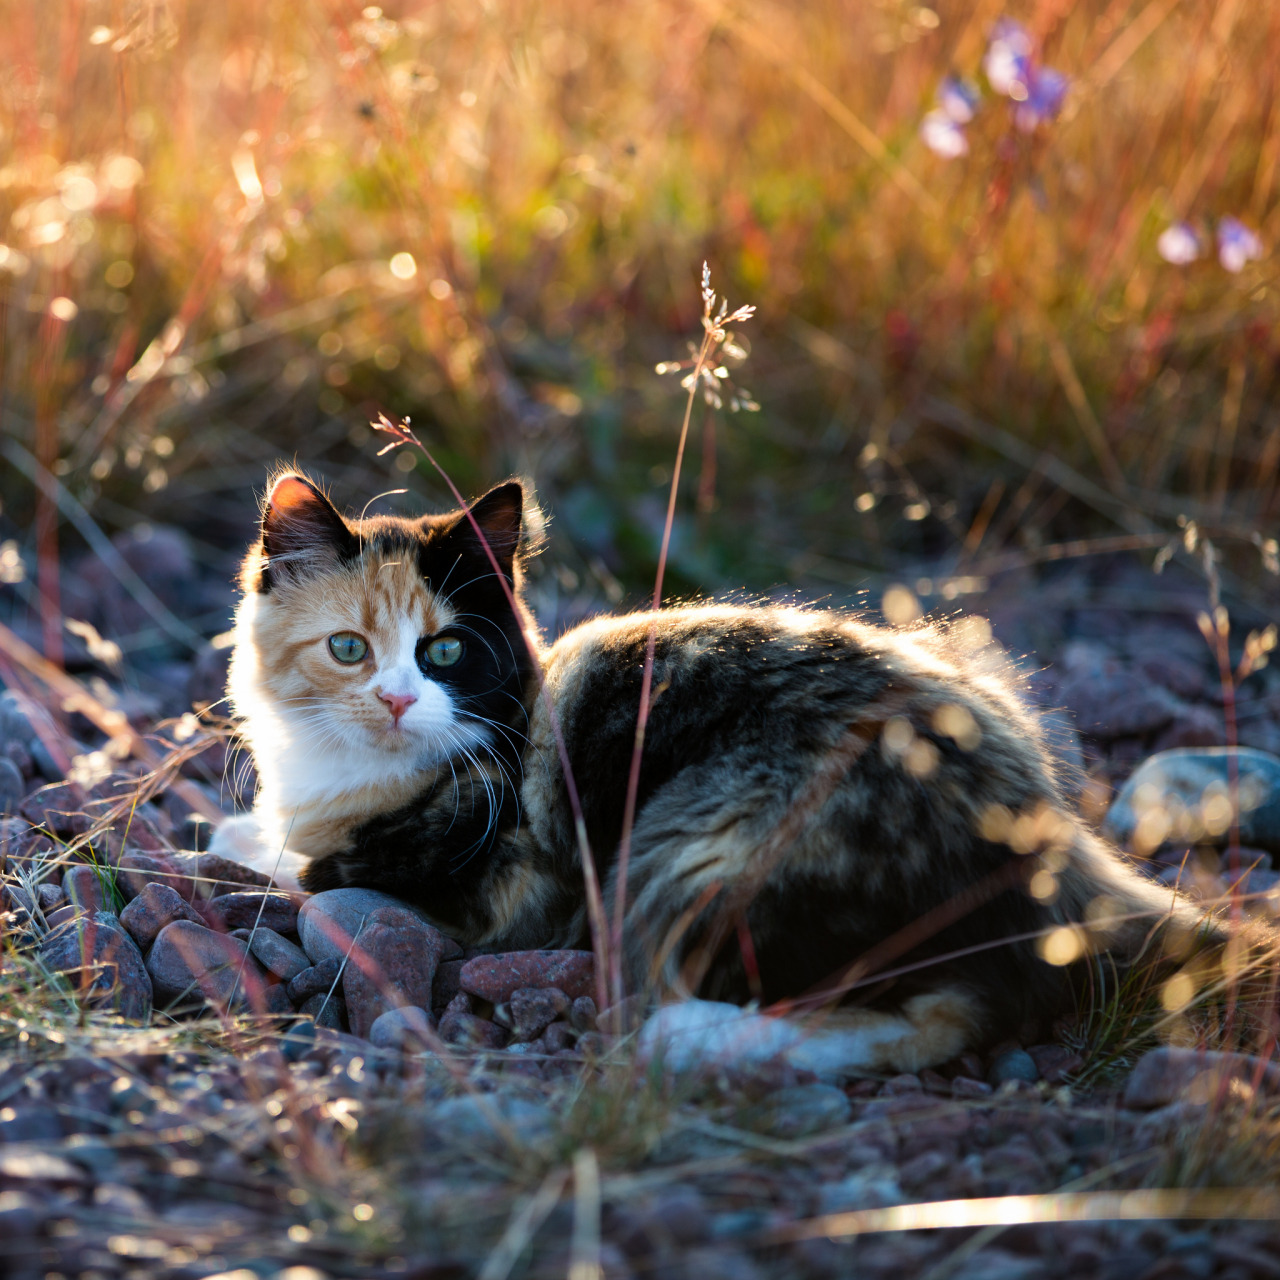
\includegraphics{Pictures/FrontCover.jpg}}} % Image background
\centering
\vspace*{11.3cm}
\par\normalfont\fontsize{35}{35}\sffamily\selectfont

\begin{center}
    % List of Latex Colour names here: https://www.overleaf.com/learn/latex/Using_colours_in_LaTeX
    \textbf{\color{Apricot} \mytitle}  % Modify the name of the colour used to suit your image
    
    \textbf{\color{White}(\ILMCode)} % Modify the name of the colour used to suit your image
    
    \color{black}ILM\par % Modify the name of the colour used to suit your image
    
    \vspace*{0.5cm}
    \color{Apricot}\author % Modify the name of the colour used to suit your image
    
    (\id)\par  
\end{center}

\endgroup

%----------------------------------------------------------------------------------------
%	COPYRIGHT PAGE
%----------------------------------------------------------------------------------------


\newpage
~\vfill
\thispagestyle{empty}

\noindent \textbf{Why taking notes like this?}
\vspace{0.5cm}

\noindent Well damn, i just want to have notes that i can read easily, are non-judgemental
and let you learn at your own page, this is by no means better than a specialized textbook,
made by an actual professional with a degree in physics or some other natural science that just
so happens to involve physics. 

\vspace{1cm}

\noindent \textbf{Can i use this text in some way?}
\vspace{0.5cm}

\noindent I mean, as long as you're conscious of it's limitations and are able to work around them, i see
no reason why i would get angry about you using this text for your own means, just remember to do no harm.

\vspace{1cm}

\noindent \textbf{There's a mistake in this book! What do i do?}
\vspace{0.5cm}

\noindent Tell me what it is, just let me know and maybe even correct it yourself, i have
no reservations on making changes in case it happens to be necessary or otherwise useful.

\vspace{1cm}

\noindent \textbf{Can i share this?}
\vspace{0.5cm}

\noindent Go ahead! These notes are open source, everybody should be able to access them i think.

\vspace{1cm}

\begin{flushright}
    \textit{(Shoutout to Yenny Hernandez, who i studied physics with @Uniandes.)}
\end{flushright}


\noindent \textit{First release, \date} % Printing/edition date

%----------------------------------------------------------------------------------------
%	TABLE OF CONTENTS
%----------------------------------------------------------------------------------------

\chapterimage{Heading1.jpg} % Table of contents heading image

\pagestyle{empty} % No headers

\tableofcontents % Print the table of contents itself

%\listoftables %uncomment this if you want to print the list of tables at the start

\pagestyle{fancy} % Print headers again


%----------------------------------------------------------------------------------------
%	Glossary
%----------------------------------------------------------------------------------------

\chapterimage{Heading1.jpg} % Table of contents heading image

\printglossaries



%----------------------------------------------------------------------------------------
%	First set of related questions
%----------------------------------------------------------------------------------------

\chapterimage{Heading2.jpg}
\chapter{The process of learning physics.}

\section{So, how \textbf{AND WHY} do we learn physics, anyways?}
\begin{flushright}
    \textit{(...like, really, why?)}
\end{flushright}

Eh, it depends.

\noindent In reality, the process of learning physics is also the process of learning how to 
observe a phenomenon in a bunch of ways. It's an experimental science that is concerned with the
study of energy, materials and their mutual interactions. We can explain a bunch of things regarding
the way our universe works with it. 

In any case, learning physics is not a marathon, cramping before an exam stresses me out, and it probably does
to you too. And we should try to learn it bit by bit, going through topics slowly and surely. Rome wasn't built in
a day, and neither should you try to learn a solid understanding in one.

When learning physics, remember:
\begin{itemize}
    \item \textbf{Do exercises.} You shouldn't try to just learn by reading the notes of some other
    guy, you might not even know me. It's 
    \item \textbf{Be critical of your own solution.} you won't always have problems right your first time
    around. If something doesn't seem to make sense, it's because it is probably not right. 
    (you probably shouldn't be getting a negative speed of light velocity when trying to calculate a bike going in a
    straight line, for example)
    \item \textbf{Understand the topics enough to explain them to someone else.} If you can teach physics to
    someone else, you will probably understand it a lot better yourself, give it a try!
    \item \textbf{Be prepared.} Check your notes, do your homework, and try to study by yourself. Prepare the things that
    you need to learn before learning them becomes a point of stress.
    \item \textbf{You're not alone.} Look for help when you need it, it's not shameful.
\end{itemize}

\vspace{20px}

\section{Important considerations.}

%----------------------------------------------------------------------------
%	Second chapter
%----------------------------------------------------------------------------

\chapter{Measurements.}



\section{Uncertainty}

There is always a level of uncertainty when measuring an object, given by the instrument of
measurement we use, an atomic clock is not the same as your uncle's watch, and even though they both
measure time, there's a certain level of uncertainty caused by the device, keep it in mind when doing experimental
work. We can express this with the symbol ' $\pm$ '

for example, if we had a milimeter of uncertainty on a measurement of 9,5 cm,
we could indicate it as such:
\begin{equation}
    l = 9,5 \pm 0,1 cm
\end{equation}

\section{Scientific Notation}

It is usual to measure both inmense and infimal quantities of mass, time, or any other thing.
For that, we shall apply the scientific notation, both on this book and elsewhere. 

\subsubsection{EXERCISES}

\paragraph*{How many years older will you be in a thousand million seconds?}

We'll start by measuring how many seconds there are in a year.

$ \frac{1 min}{60 s} * \frac{1 h}{60min} * \frac{1 d}{24 h} * \frac{1 yr.}{365 d} = 1x10^9 s $

And now we'll take our given time on years

$ time = 1,000,000s * 1,000s = 1000x10^6 s $

\textbf{Answer:}$ 31 yrs. $


\paragraph*{How many nanoseconds does the speed of light need to travel 1ft in the void?}

$ 1 ft = 30,48 cm $

Even though not specifically notified in the exercise, we must remember that:

\begin{gather}
    1m = 100cm    
\end{gather}

\section{Types of units}
In the realm of physics, there is a bunch of ways to categorize units, be it by what do they 
measure or how do they measure it

\section{Scalar units}

A scalar unit is defined as an unit with magnitude, but no direction. Such measurements
aren't really concerned with being tied with a specific force acting over a particle. 

Examples of such units include:
\begin{itemize}
    \item Natural numbers.
    \item Constants.
    \item Acceleration
\end{itemize}

\section{Vectors}

A vector is a measurement with both a magnitude and a direction. that can exist on
a specific set of dimensions. On this course, we won't be concerning ourselves with hyperplanes
and might sparingly cover 3-dimensional planes, they would both be useful for you to learn eventually, so i encourage
you to learn about them on your own accord, however. Our examples will be two-dimensional, for a simple, 
introductory example, consider the following vector; $ \vec{A} = 
\begin{pmatrix}
    3 \\
    2
\end{pmatrix} $ :

\begin{center}
 \includegraphics*[scale=0.5]{vec_1.png}

 \textit{Vector with x coordinates '3' and y coordinates '2'}
\end{center}


This is what we call a cartesian vector, for it's magnitudes are defined by the coordinates in a
cartesian plane, however, we can turn it into a polar vector, measured by it's magnitude and 
angle, through the following formulas:

\begin{gather}
    |\vec{A}| = \sqrt{A_x^2+A_y^2} \\
    \tan \theta = \frac{A_y}{A_x}
\end{gather}

\paragraph{Exercise: Turning our example vector 'A' into a Polar vector.}
\textit{Magnitude}
\begin{gather}
    |\vec{A}| = \sqrt{3^2+2^2}
    |\vec{A}| = \sqrt{9+4} = \sqrt{12} = 2\sqrt{3} 
\end{gather}
\textit{Angle}
\begin{gather}
    \tan \theta = \frac{2}{3} \\
    \theta = \tan^-1(\frac{2}{3}) \\
    \theta = 33,69^o 
\end{gather}

\noindent Equally, we can turn a polar vector into a cartesian one. 

So, given an angle $ \theta $ and a magnitude $ |\vec{A}| $, we can suppouse the measurements of a two-directional vector as:
\begin{gather}
    A_x  = |\vec{A}| \cos \theta \\
    A_y = |\vec{A}| \sin \theta
\end{gather}

And given this, we can consider the vector '$\vec{A}$' as, $ \vec{A} = A_x i + A_y j $, where 'i' and
'j', are what we're going to call a \textbf{unit vector}, a vector in a specific direction that has a value of 1.
(this is considered an identity value for multiplication operations, and lets us do some vector sum 
operations more intuitively)


\paragraph{Exercise: Turning our example vector 'A' back into a cartesian vector.}
\begin{gather}
    A_x  = |2\sqrt{3}| \cos 33,69^o = 2,88 \approxeq 3 \\
    A_y = |2\sqrt{3}| \sin 33,69^o = 1,92  \approxeq 2
\end{gather}

As it might be evident, the conversion isn't exact, this happens because of the 
angle not being an exact conversion, this will happen when you disregard part of a value
for whatever reason. The more exact of a measurement you keep, the less uncertainty you will
end up with.

\subsection{Vector sum}


We can take any $ \vec{a} $ and $ \vec{b} $ vectors on the same space and add them to each other
in the form:

\begin{equation}
    \begin{bmatrix}
        a_1 \\
        a_2 \\
        a_3 \\
    \end{bmatrix}
    +
    \begin{bmatrix}
        b_1 \\
        b_2 \\
        b_3 \\
    \end{bmatrix}
    = 
    \begin{pmatrix}
        a_1 + b_1\\
        a_2 + b_2\\
        a_3 + b_3\\
    \end{pmatrix}
\end{equation}

Such form remains in the case we can do subtraction, which is expressed on the equation:

\begin{equation}
    \begin{bmatrix}
        a_1 \\
        a_2 \\
        a_3 \\
    \end{bmatrix}
    -
    \begin{bmatrix}
        b_1 \\
        b_2 \\
        b_3 \\
    \end{bmatrix}
    = 
    \begin{pmatrix}
        a_1 - b_1\\
        a_2 - b_2\\
        a_3 - b_3\\
    \end{pmatrix}
\end{equation}

This kind of operations have certain properties, shown as:
\begin{gather}
    (\alpha + \beta)\vec[v] = \alpha\vec{v} + \beta\vec{v} \\
    \vec{v} * 1 = \vec{v} \\
    \vec{v} * \vec{0} = \vec{0} \\
    \beta \vec{v} = 
    \begin{pmatrix}
        \beta a_1\\
        \beta a_2\\
        \beta a_3\\
    \end{pmatrix}
\end{gather}

Two vectors $ \vec{a} $ and $ \vec{b} $ are equal if and only if:
\begin{equation}
    \begin{cases}
        \vec{a} \exists \mathbb{R}^3 \\
        \vec{b} \exists \mathbb{R}^3
    \end{cases}
    \implies
    \begin{pmatrix}
        a_1 = b_1\\
        a_2 = b_2\\
        a_3 = b_3\\
    \end{pmatrix}
    \text{
        \textit{note: this can be generalized to 'n' dimensions larger than 0}}
\end{equation}

in either case,  $ \vec{0} $ is the identity of the operation, therefore:
\begin{equation}
    \vec{a} + \vec{0} = \vec{a}
\end{equation}


\subsection{Scalar/dot product}
We can multiply vectors between each other with the following formula:

$$ |\vec{A}| \centerdot |\vec{B}| = |\vec{A}||\vec{B}|\cos \theta $$

We can also write it as such for cartesian vectors:
$$ A_x B_x + A_y B_y + A_z B_z $$

This is a commutative operation, that won't be affected by neither A nor B's 


\subsection{Cross/Vectorial product}

We can define the formula for the cross product of two vectors in a 3-dimensional space
as:
\begin{equation}
    \vec{A} x \vec{B} = 
    \begin{pmatrix}
        (A_y - B_z - A_z B_y) i \\
        (A_x B_z - B_x A_z) j \\
        (A_x B_y - B_x A_y) k   
    \end{pmatrix}
\end{equation}

This will come handy when studying Torque;

\subsection{Solved Exercises}
\subsubsection{Vector Sum}
\paragraph{An espeologist explores a cave and follows a }

\subsection{Dot/Cross Product}


\subsection{Scientific Notation}
\paragraph{how many nanoseconds does a ray of light require to travel 3 meters in the void?}

\textit{Solution}


\paragraph{Estimate how many gallons of gasoline are consumed by private cars in Colombia in a year.
Assume that on average there is one car for every 10 inhabitants and that on average each car travels $10^4$ km per year, with an average engine efficiency of 25 km/gallon.}

\indent \textit{Solution.}
\begin{gather}
    \text{Population of Colombia as of 2020}= 51520000 \\
    \text{Number of cars}= 51520000/10 = 5152000 \text{ } cars\\
    \text{Kilometers traveled}=5152000 \text{ } cars * 10^4 \frac{km}{yr} = 51520000000\frac{km}{yr} = 5,152x10^{10}\frac{km}{yr}\\
    \text{Gallons per year}= \frac{5,152x10^{10}\frac{km}{yr}}{25\frac{km}{gallon}}=2060800000\frac{\text{gallon}}{yr} = 2,0608x10^{9}\frac{\text{gallon}}{yr}
\end{gather}

%----------------------------------------------------------------------------
%	More sections?
%----------------------------------------------------------------------------

% Simply upload additional images Heading5.jpg, Heading6.jpg etc. into the pictures folder

\chapterimage{Heading4.jpg}
\chapter{Basic Kinematics}

\section{One-Dimensional Movement}
One-dimensional movement is probably the most basic kind of movement, as unbound by the expectations of 
more than two directions to move to, it allows itself to simply define the route from a point 'A' to a 
point 'B' in a straight line. 



Such movement can be defined as:
\begin{equation}
    \Delta x = x_2 - x_1   
\end{equation}

medium velocity on this kind of movement can be calculated as:

\begin{equation}
    v_{med} = \frac{\Delta x}{\Delta y} = \frac{x_2 - x_1}{t_2 - t_1}
\end{equation}

Keep in mind, we can define negative velocity in such systems to move in a
negative direction (i.e moving from B=7 to A=3, for example.) and besides that
\textbf{This is not the same as speed, because speed is concerned with how fast the object moves
while this is concerned with how fast the object arrives somewhere, and that's not the same.}

\section{instantaneous speed and velocity}

It should now be evident that we can assume a straight line that can be interpreted as the velocity of an
object, as we could see in this two-dimensional graph.

\begin{center}
    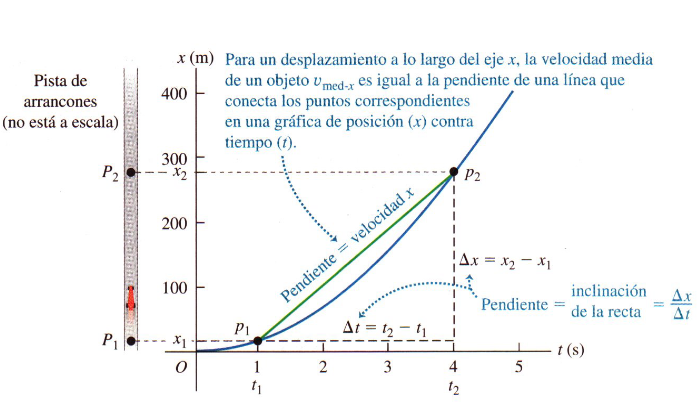
\includegraphics[scale = 0.6]{pendant.png}    
\end{center}

We define the instantaneous velocity of an object as a derivative of the form:
\begin{equation}
    v = \lim_{\Delta t \to 0} \frac{\Delta x}{\Delta t} = \frac{dx}{dt}   
\end{equation}

The simplest formula for such a calculation is, however:

\begin{equation}
    x = x_0 + vt
\end{equation}


\section{Acceleration}

Of course, not all objects will move at a constant pace, most times there will be a 
change in speed happening at some moment in their movement. This is a scalar 
variable that can be used to calculate the overall distance when taking into account
such changes on movement. We can calculate the acceleration of an object as follows:

\begin{equation}
    a = \frac{\Delta v}{\Delta t}
\end{equation}

we can integrate distance as a function of acceleration as it follows, as well:

\begin{equation}
    \int_{t}^{0} v \,dt = \int_{x}^{x_0} \,dx \\ \text{\textit{ Note: we can integrate the result of this equation to prove correctness.}}
\end{equation}

Through a mathematical proof that 

\subsection{Constant Acceleration}

An object can be said to have constant acceleration when acceleration is not a variable, but a 
constant. When working on such a system we can affirm velocity as:

\begin{equation}
    at = v - v_0
\end{equation}

and we can indicate distance as:

\begin{equation}
    x = x_0 + v_0 t + \frac{1}{2} at^2
\end{equation}

From these two we can gather the following formulas:

\begin{itemize}
    \item $v = v_0 + at$
    \item $t = \frac{v-v_0}{a}$
    \item $ v^2 = v^2_0 + 2a(x-x_0) \text{\textit{If we don't know time}} $
    \item $ x - x_0 = (\frac{v+v_0}{2})t \text{\textit{If we don't know acceleration}} $
\end{itemize}

\section{Two-dimensional movement}

Again, this is a pretty self explainatory title. As it just refers to the
representation of movement in more than a two independent axis. We never were
living in a straight line anyways so it shouldn't come as a surprise to you that 
physics doesn't live there either. 

We can imagine two vectors to indicate the beginning and end of our specified movement, and yes, this
could potentially include (0,0), in any case, we can write them as:

\begin{gather}
    \vec{r_i} = x_i i + y_i j \\
    \vec{r_f} = x_f i + y_f j
\end{gather}

To describe a movement in two dimensions with these vectors, we can use the following equations:
\begin{gather}
    \Delta \vec{r} = \vec{r}_f - \vec{r}_i \\
    \Delta \vec{r} =  (x_f - x_i) i + (y_f - y_i) j 
\end{gather}

we can also affirm:

\begin{gather}
    |\vec{r_i}| = \sqrt{x_i^2 + y_i^2} \\
    \theta = \arctan(\frac{y_i}{x_i}) \\
    \vec{r_i} = |\vec{r_i}| \cos \theta i + |\vec{r_i}| \sin \theta j
\end{gather}

These are just vectorial operations, and they apply for either vector, nothing really changes from
how we already expected vectors to work. 


\subsection{Projectile movement.}

We can assume, on this version of a two-dimensional movement, that:

\begin{gather}
    x = x_0 + v_0 \cos \theta t \\
    v_x = v_0 \cos \theta_0 = v_0 x \\
    y = y_0 + v_0 \sin \theta_0 t - \frac{1}{2} gt^2 \\
    v_y = v_0 \sin \theta - gt \\
    v_y^2 = v_0^2 \sin^2 \theta_0 - 2g (y - y_0)
\end{gather}

We can also assume an 'R' distance that will be the maximum possible distance in the x axis
with 'y' as 0. We can get it as:

\begin{gather}
    v_0 \sin \theta_0 = gt \\
    t = \frac{v_0 \sin \theta_0}{g} \\
    R = 0 + v_0 \cos \theta_0 \centerdot \frac{2 v_0 \sin \theta_0}{g} \\
    R = \frac{v_0^2 \sin(2 \theta_0)}{g}
\end{gather}

This is the maximum possible distance that you can get for a displacement given 
certain parameters to be replaced in such a formula. Keep in mind that when $\theta$ is 45 degrees, the
value of 'R' is at its peak for that specific configuration, so given a question regarding angles, the closest to
45 it is, the furthest it will make it. A few other useful formulas are:

\begin{gather}
    x = x_0 + v_0t \\
    y = h + v_0 \sin \theta_0 t - \frac{1}{2} gt^2 \\
    t = \sqrt{\frac{2h}{g}} \\
    x = v_0 \sqrt{\frac{2h}{g}}
\end{gather}

When working on an elevated end point, we can imagine that, given a distance 'D' and an elevated endpont 'H':

\begin{gather}
    x = x_0 + v_0 \cos \theta_0 t \\
    y = y_0 +v_0 \sin \theta_0 t - \frac{1}{2} gt^2 \\
    v_y^2 + v^2 \sin^2 \theta_0 -2g(y - y_0) \\
    D = v_0 \cos \theta_0 t \\ 
    t = \frac{D}{V_0 \cos \theta_0} \\
    H = \frac{v_0 \sin \theta_0 D}{v_0 \cos \theta_0} - \frac{1}{2} g (\frac{D^2}{v_0^2 \cos^2 \theta_0}) \\
    H = D \tan \theta_0 - \frac{1}{2} g \frac{D^2}{v_0^2 \cos^2 \theta_0} \\
    V_0^2 = \frac{gD^2}{2 \cos^2 \theta_0 (D \tan \theta_0 - H)}
\end{gather}

\paragraph*{What's the secret on getting these problems right?}

Writing all of the possible equations and looking at:

\begin{itemize}
    \item What do i have?
    \item What do we need?
    \item How can i rewrite the equations that i have in order to get what i need?
\end{itemize}

\section*{Circular Movement}

\begin{gather}
    \Delta s = R \Delta \phi \\ 
    \frac{\Delta s}{R} = \frac{|\Delta v|}{v_1} \\
    |\Delta v| = v_1 \Delta \phi \\
    a = \frac{v^2}{r} \\
    v = \frac{2 \pi R}{T} \\
    T = \frac{2 \pi R}{v}
\end{gather}

\section{Exercises}
\subsection*{One-dimensional movement}


\subsection{Acceleration}
\paragraph{what's the maximum possible height of a marker being thrown at a
velocity of $ 0,5 \frac{m}{s}$ ?}

We know that:
\begin{itemize}
    \item gravity (acceleration): $ -9,8 \frac{m}{s^2} $
    \item initial position: 0
    \item initial velocity = $ 0,5 \frac{m}{s} $
\end{itemize}

\begin{gather}
    v^2 = v^2_0 + 2a(x-x_0) \\
    0 = v_0^2 - 2g(y-0) \\
    v_0^2 = 2gy \\
    y = \frac{v_0^2}{2g} \\ 
    y = - \frac{0,5\frac{m}{s}^2}{2(9,8\frac{m}{s^2})}
\end{gather}


\chapter{Newton's laws of motion}

Newton's laws of motion are three basic laws of classical mechanics that describe the relationship between the motion of an object and the forces acting on it.

\section{Forces.}

We mostly can assume forces to mantain the following

\begin{gather}
    \vec{R} = \vec{F}_1 + \vec{F}_2\\
    \vec{R} = \vec{R}_x i + \vec{R}_y j\\
    \vec{R}_x = \vec{F}_{1x} + \vec{F}_{2x} \\
    \vec{R}_y = \vec{F}_{1y} + \vec{F}_{2y}
\end{gather}

\section{Newton's laws.}

\subsection{First Law}

A body in state of rest, or in uniform motion in a straight line
will have an overall summatory of forces equal to 0

\begin{equation}
    \sum \vec{F} = 0
\end{equation}

\subsection{Second Law}

A net force that acts over a body makes it accelerate in the same direction
as the net force. The magnitude of acceleration is directly proportional
to the magnitude of the forces acting over it.

\begin{itemize}
    \item if a net force acts over a body, this body accelerates
    \item The direction of acceleration is the same as a net force.
\end{itemize}

we can assume:
\begin{gather}
    \vec{F}_{net} = m \vec{a} \\
    \vec{F} = \frac{d \vec{p}}{dt} 
\end{gather}

\subsection{Third Law}

When two bodies interact their forces are always equal in magnitude and
opposed in direction. This can be expressed as:

\begin{equation}
    \vec{F} AB = - \vec{F} BA
\end{equation}

\section{Free-body diagrams}

A free body diagram is a representation of a system and the forces acting over it.

\section{Friction}

Friction is the 

\section{Drag and Terminal Velocity}

there is a force that linearly depends on velocity called drag. Such 


\section{Examples}
\subsection{Forces}

\paragraph{Two horses horizontally pull strings tied
to a tree trunk. The forces $\vec{F}_1$ and $\vec{F}_2$
are applied such as  $\vec{R}$ has the same magnitude as $\vec{F}_1$ 
and is $90^o$ from $\vec{F}_1$; if $\vec{F}_1 = 1300N$, calculate
the magnitude of $\vec{F}_2$ and it's direction.}

\textit{Solution}

\paragraph{An electron with mass $9,11x10^{-31} kg$ goes from
a kinescope with an initial speed of 0 and travels in a straight line to
an end point 1,80 cm away. arriving with a speed of $ 3x10^{6} \frac{m}{s} $.
if net force is constant, calculate acceleration, time, and net force (in Newtons).}

\textit{solution}

We know:
\begin{itemize}
    \item $ V_f = 3x10^6 \frac{m}{s} $
\end{itemize}

\textit{Acceleration}

\begin{gather}
    \vec{V}_f^2 = \vec{v}_0^2 + 2ad\\
    \vec{V}_f^2 = \vec{v}_0^2 + 2a(x-x_0) \\
    a = \frac{\vec{V}_f^2}{2d}\\
    a = \frac{3x10^6 \frac{m}{s}}{2 x 1,8x10^{-2}m} = 2,5x10^{14} \frac{m}{s^2}
\end{gather}

\paragraph{A 2.00 kg object is subject to three forces that give it a total
acceleration of $\vec{a} = -(8,00 \frac{m}{s^2})i + (6,00 \frac{m}{s^2})j$; given that two of the three forces are
$ (30,00N)i + (16,00N)j $ and $-(12,00N)i + (8,00N)j$, What is the third force?}

\textit{solution}

We know that:
\begin{gather}
    \sum F_x = ma_x\\
    \sum F_y = ma_y
\end{gather}

and therefore:
\begin{gather}
    \sum{F_x} = (2,00 kg)*(-8,00 \frac{m}{s^2}) = -16N \\
    \sum{F_y} = (2,00 kg)*(6,00 \frac{m}{s^2}) = 12N \\
    F_{x1} + F_{x2} + F_{x3} = -16N\\
    F_{y1} + F_{y2} + F_{y3} = 12N\\
    <replace>\\
    30,0N - 12,00N + F_{x3} = -16N\\
    16,00N + 8,00N + F_{y3} = 12N\\
    F_{x3} = -16N + 12,00N - 30N\\
    F_{y3} = 12N - 8,00N - 16,00N\\
    F_{x3} = -34N\\
    F_{y3} = -12N
\end{gather}

\paragraph*{An ice block that weighs 8,00kg is liberated from rest through a 
ramp with no friction with a length of 1,50m. It slides downwards and reaches a
maximum velocity of 2,50 m/s when finishing its slide.}
\begin{gather}
    \sum_{y} = N - mg \cos \theta = 0\\
    \sum_{x} = -mg \sin \theta = -ma\\
    a = g \sin \theta
\end{gather}

\textit{What's the angle of the ramp?}
\begin{gather}
    v_f^2 = v_i^2 + 2ad\\
    2,5 \frac{m}{s}^2 = 0 \frac{m}{s} + 2ad\\
    2,5 \frac{m}{s}^2 = 2 \centerdot 1,50 m (9,8 \frac{m}{s^2} \sin \theta)\\
    \frac{2,5 \frac{m}{s}^2}{2 \centerdot 1,50 m} = 9,8 \frac{m}{s^2} \sin \theta\\
    \theta = \arcsin{(\frac{2,5 \frac{m}{s}^2}{2 \centerdot 1,50 m \centerdot 9,8 \frac{m}{s^2}})}\\
    \theta = 4,87^o
\end{gather}


\textit{What's the speed the ice would have if there was a friction force of 10N rarallel to the surface?}
\begin{gather}
    \sum_{y} = N - mg \cos \theta = 0\\
    \sum_{x} = -mg \sin \theta = -ma + f_k\\
\end{gather}

\chapter{Work}

Work is the exertion of forces over a body, that moves from one point to another.

\begin{gather}
    \vec{F} = \ forces\\
    s = \  movement
\end{gather}

So, to measure how effective a force is over a moving object, we must first decide:

\begin{itemize}
    \item Magnitude
    \item Direction
\end{itemize}

We must therefore, understand that only components that are parallel to the movement itself are effective. 

Given this, we can affirm:

$$W = F_{||}s = F(\cos{\phi})s = Fs \cos{\phi} $$

or, our work is equal to the forces parallel to our movement. We can also derive from it, that work will be a 
dot product between the vectors acting, set up as $\vec{F} \cdot \vec{s}$. Let's remember a few things about this sort of
operation
\begin{itemize}
    \item The result is a scalar number in $\mathbb{R}$
    \item we have two ways to calculate it: $$
    \begin{cases}
        \vec{F} = F_x i + F_y j + F_z k = (F_x, F_y, F_z)\\
        \vec{s} = \Delta_x i + \Delta_y j + \Delta_z k \\
    \end{cases} \ implies \vec{F} \cdot \vec{s} = F_x \Delta_x + F_y \Delta_y + F_z \Delta_z
    $$
    When we have the components, and:
    $$
    \begin{cases}
        F = |\vec{F}|\\
        s = |\vec{s}|
    \end{cases} \implies \vec{F} \cdot \vec{s} = Fs \cos{\phi}
    $$ When we don't, $\phi$ is the angle between both vectors.
    \item $0 \leq \phi \leq 90^o$
    \item Work is an energy transference, positive if towards the system and negative if coming from it.
\end{itemize}

\section{Theorem of Work and Kinetic Energy}

An object that moves with constant acceleration and over it 

$\vec{W} = F \Delta x$

$W = \frac{1}{2}mv^2 - \frac{1}{2}mv_0^2$

\section{Work by variable forces}
When a force is variable, then we can affirm:
\begin{gather}
    \Delta W_i = F_{x,i} \Delta x_i\\
    W_T = \sum_i F_{x,i} \Delta x_i\\
    \lim_{\Delta x \to 0} \sum_i F_{x,i} \Delta x_i = \int_{x_i}^{x_f} F_x dx\\
    W = \int_{x_i}^{x_f} F_x dx \cos{\phi}\\
    W = \int_{i}^{f} \vec{F} \cdot d\vec{s}
\end{gather}

\section{Hooke's Law}

The work made by an elastic force is:

\begin{gather}
    F = k\vec{x}
\end{gather}

And:

\begin{gather}
W_s = \frac{1}{2}k x_f^2 - \frac{1}{2} k x_i^2
\end{gather}

\section{Curved trajectory work.}

\begin{gather}
    F = w \tan{\theta}\\
    s = r \theta \\
    W = mg \tan{\theta} ( R \theta )
\end{gather}

\section{Potency}

When a force is constant, we can say 

\begin{gather}
    P = \frac{dW}{dt} = \frac{F \cos \phi dx}{dt} = F cos \phi(\frac{dx}{dt})\\
\end{gather}

\section{Potential Energy}

Potential energy is the associated energy to the configuration of
a system of objects that interact between themselves. This can be, for example;
expressed as either:

\begin{itemize}
    \item Gravitational potential energy:
    \begin{equation}
        \Delta U = - \int_{y_i}^{y_f} - mg dy
    \end{equation}
    \item Elastic potential energy
    \begin{equation}
        \Delta U = - \int_{x_i}^{x_f} - kx dx
    \end{equation}
\end{itemize}

Such a concept allows us to write, besides our previous definition of the work-energy theorem $W = \Delta k$, A
different, alternative definition:

\begin{equation}
    W = - \Delta U
\end{equation}



\section{Examples.}

\paragraph{A}

We know that:
\begin{gather}
    W = 12J\\
    W = \frac{1}{2} k (3 x 10^{-2}m)^2 - \frac{1}{2} k x_i^2\\
    24J = k(3 x 10^{-2}m)^2\\
    k = 2,7 x 10^4 \frac{N}{m}
\end{gather}

Therefore:
\begin{gather}
    F = kx\\
    F = 810 N\\
    fr = -kx\\
    F + fr = 0\\
    W = \frac{1}{2} k (-4 x 10^{-2})^2\\
    W = \frac{1}{2} 2,7 x 10^4 \frac{N}{m} \cdot 16 x 10^{-4} m^2\\
    W = 21,6 J 
\end{gather}

\paragraph{B:}

We can assume:
\begin{gather}
    F_x = -[20N + 3 \frac{N}{m} x]\\
    \int_0^{6,9m} = F dx
\end{gather}

Therefore:

\begin{gather}
    \int_0^{6,9m} -[20N + 3 \frac{N}{m} x] dx = -209.4 J
\end{gather}

\paragraph*{a 250g block is let fall }

\begin{gather}
    W_g = mg x \cdot \cos{0}\\
    W_g = mgx \\
    W_g = 0.3J\\
    W_k = \frac{1}{2} k x^2\\
    W_k = 1,8 J\\
    \frac{1}{2} mv^2 + mgx = \frac{1}{2}kx^2\\
    \frac{1}{2}mv^2 = 1,5J\\
    v = 3,47 \frac{m}{s}
\end{gather}

And, for the theoretical of the 'd' literal:

\begin{gather}
    v_i = 2(v_0)\\
    \frac{1}{2}m(2 v_0)^2 + mgx_2 =\frac{1}{2} kx_2^2\\
    \frac{1}{2} k x_2^2 - mgx_2 - 2 mv_0^2 = 0
    x_2 = 22,9 cm
\end{gather}

\paragraph*{a 2kg piece of wood is let slide through figure 1: both curved sides are
perfectly smooth, but the bottom is coarse and has a longitude of 30m. The coefficient of kinetic friction is 
0.2 against wood. The piece has an initial height 4m above the coarse bottom.}

\begin{center}
    \textit{Figure 1}
\end{center}

\begin{gather}
    mgh = \frac{1}{2}mv_1^2\\
    W_f = \mu_k mg x \cos{180}\\
    W_f  = - \mu_k mg x\\
    W_f = \Delta k  = \frac{1}{2} m v_f^2 - \frac{1}{2}mv_1^2 \\
    - \mu_k mg x  = - \frac{1}{2} m2gh \\
    x = \frac{h}{\mu_k}
\end{gather}

\paragraph{Coarse spring:}

\begin{gather}
    \frac{}{}
\end{gather}

\chapter{Momentum and Collisions}

Linear momentum is a vectorial quantity that can be measured as:

$\vec{p} = m\vec{v}$

The second law of Newton can be written in respect to momentum, and 

\section{Collision and Impulse}

In a collision, the external force on the body is brief, considerable in magnitude and
short in effect over the system, it changes the linear
changes the linear momentum of the system suddenly and can be seen as:

\begin{equation}
    d \vec{p} = \vec{F} (t) dt
\end{equation}

\section{Conservation of linear momentum}

\section{Second Law of Newton on a particle system}

Let:

\begin{equation}
    \vec{F}_{net} = M \vec{a}_{c.o.m}
\end{equation}

We can then affirm:

\begin{itemize}
    \item Net force will be the summatory of all external forces acting over the
    body
    \item M is the total mass of the system; no mass gets out of the system if the system is closed
    \item $\vec{a}_{c.o.m}$ is the acceleration of the center of mass in the system. 
\end{itemize}

\section{Examples}

\paragraph{A ball weighing 1.2 kg is dropped vertically on a
vertically on a floor, reaching the ground
the ground with a speed of 25m/s. The ball
bounces with an initial speed of 10 m/s a)
What impulse acts on the ball during
the contact? b) If the ball is in contact
with the ground for 0.020 s what is the
magnitude of the average force on the
floor from the ball?}

\begin{gather}
    p_i = m v_i j\\
    p_f = m v_f j \\
    \Delta p = p_f - p_i = (m v_f - (-mv_i))\\
    \Delta p = p_f - p_i = mv_f + mv_i = m(v_f + v_i) \\
    J = \Delta p = m(v_f + v_i)\\
    J = \int_{t_i}^{t_f} F dt \\
    = F (t_f - t_i) \\
    F = \frac{J}{t_f - t_i} 
    \Delta p = 42 kg \frac{m}{s}\\
    F = 2100 N
\end{gather}

\chapter{Rotation}

A rigid body can rotate and we can measure the way it does.

$v_i = \omega r_1$

where $\omega$ is the angular velocity and

\section{Energy in rotating bodies}

We can model energy in a rotating body as:

\begin{equation}
    K = \frac{1}{2} \omega^2 \sum_i m_i (r_i)^2
\end{equation}

This can also be written as:

\begin{equation}
    K = \frac{1}{2} I \omega^2
\end{equation}

Because the sum can be rewritten as the Inertia momentum of the object we're modeling.
However, we might also model it as an integral, such as:

\begin{equation}
    I = \int_0^r r^2 dm
\end{equation}

the units should always eng up being for mass and length squared, such as:

$$ kg \cdot m^2 $$

\section{Parrallel axis theorem}
\begin{equation}
    I = I_{com}+Mh^2
\end{equation}

where 'h' is the distance to the center.

\chapterimage{Heading4.jpg}
\chapter{Useful Information}

\section{Constants}
\begin{itemize}

    \item Speed of light: 
    
    $299'792.458 \frac{km}{s}$, can be approximated to $ 3x10^8 m/s $ when you're not concerned with precision.

    \item Gravity in earth: 
    
    $ 9,81 \frac{km}{s^2}$ (A bit oversimplified, but for now it should suffice)

\end{itemize}
\section{Formulas}
\begin{itemize}
    \item Newton.
    
    $ 1N = 1 \frac{kg \centerdot m}{s} $
\end{itemize}
\section{Definitions}
\begin{itemize}
    \item Delta: 
    
    noted as $ \Delta $, it indicates change in a variable, taking $ x $ as the variable
    that changes, $ x_0 $ as it initial state and $ x_f $ as the final one, we can indicate how much it
    changes as follows: $$ \Delta x = x_f - x_0 $$
\end{itemize}
%----------------------------------------------------------------------------------------
%	References
%----------------------------------------------------------------------------------------

\chapterimage{Heading4.jpg} % Chapter heading image

\bibliographystyle{plain} % Change this to IEEE or Harvard etc.
\bibliography{references}


\end{document}